\documentclass[11pt]{article}
\usepackage[T1]{fontenc}
\usepackage[margin=0.94in]{geometry}
\usepackage{amsmath,amssymb,amsthm,mathtools}
\usepackage{graphicx}
\usepackage{microtype}
\usepackage{xcolor}
\usepackage[hypertexnames=false,colorlinks=true,linkcolor=blue!55!black,urlcolor=blue!65!black,citecolor=blue!55!black]{hyperref}

\newtheorem{theorem}{Theorem}
\newtheorem{lemma}[theorem]{Lemma}
\newcommand{\Hh}{\mathcal H}
\newcommand{\Dom}{\operatorname{Dom}}
\newcommand{\Ran}{\operatorname{Ran}}

\title{The specific isometry \(W=JV\) need not be pure}
\author{Candidate full counterexample to the open problem in arXiv:2205.15925}
\date{12 August 2026}

\begin{document}
\maketitle

\noindent
\fbox{\begin{minipage}{0.94\textwidth}
\textbf{Status: candidate full counterexample, likely valid.}
The answer to the open problem following Theorem C of Martin is negative,
even for a multiplicity-free diagonal operator.  Take
\(Ae_k=k^{-1}e_k\) on \(\ell^2(\mathbb Z\setminus\{0\})\), and apply exactly
the paper's symmetric-restriction construction using its natural symmetric
counting-measure model.  If \(A=J|A|\), the resulting pure isometry \(V\)
satisfies
\[
  JV=I
  \quad\hbox{on the infinite-dimensional subspace}\quad
  \{h:h_{-n}=-h_n\}.
\]
Consequently the construction's \(W=JV\) has a nonzero (indeed
infinite-dimensional) unitary part and is not pure.
\end{minipage}}

\section{The exact open problem}

Martin proves that if a bounded injective self-adjoint operator \(A\) is
Hankel with respect to a pure isometry \(V\) and \(AV>0\), then, writing
\(A=J|A|\), the isometry \(W=JV\) makes \(|A|\) doubly-positive Hankel.
The unitary part of \(W\), if present, must be the identity.  The subsequent
Remark 2 asks whether the \emph{specific} \(V\) built in the sufficiency
proof from a spectral restriction of \(A^{-1}\) might force \(W\) to be
pure \cite{Martin}.  The source page is reproduced below.

\begin{center}
  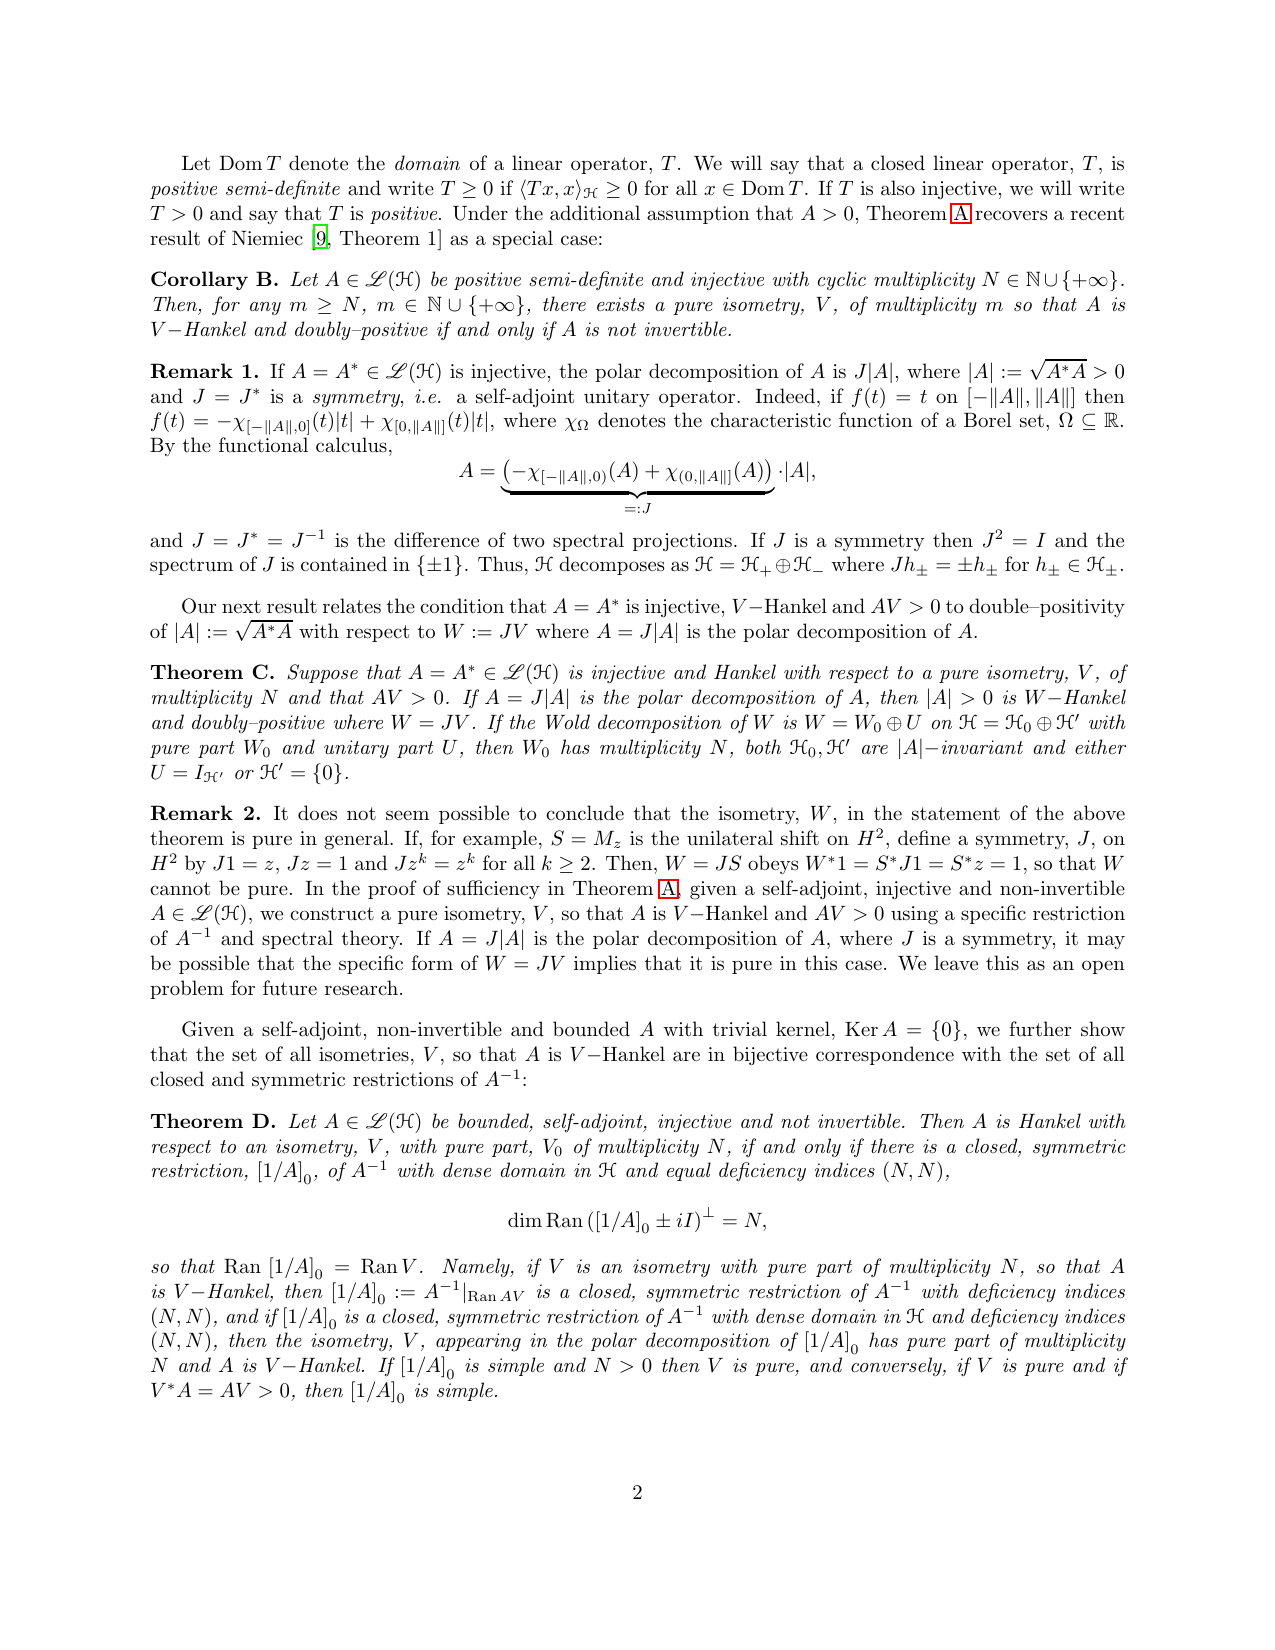
\includegraphics[height=0.78\textheight]{figures/source_open_problem.png}
\end{center}
\clearpage

The construction first represents \(A^{-1}\) as multiplication by the
independent variable on \(L^2(\mu)\), where \(\mu\) satisfies the Herglotz
condition.  It then restricts the multiplication operator to
\begin{equation}
 \mathcal D_0=
 \left\{h\in\Dom M_t:\int h\,d\mu=0\right\},
 \qquad T_0=M_t|_{\mathcal D_0},
 \tag{1}
\end{equation}
and takes the isometric polar factor \(V\) of \(T_0\).  This defining source
page is reproduced next.

\begin{center}
  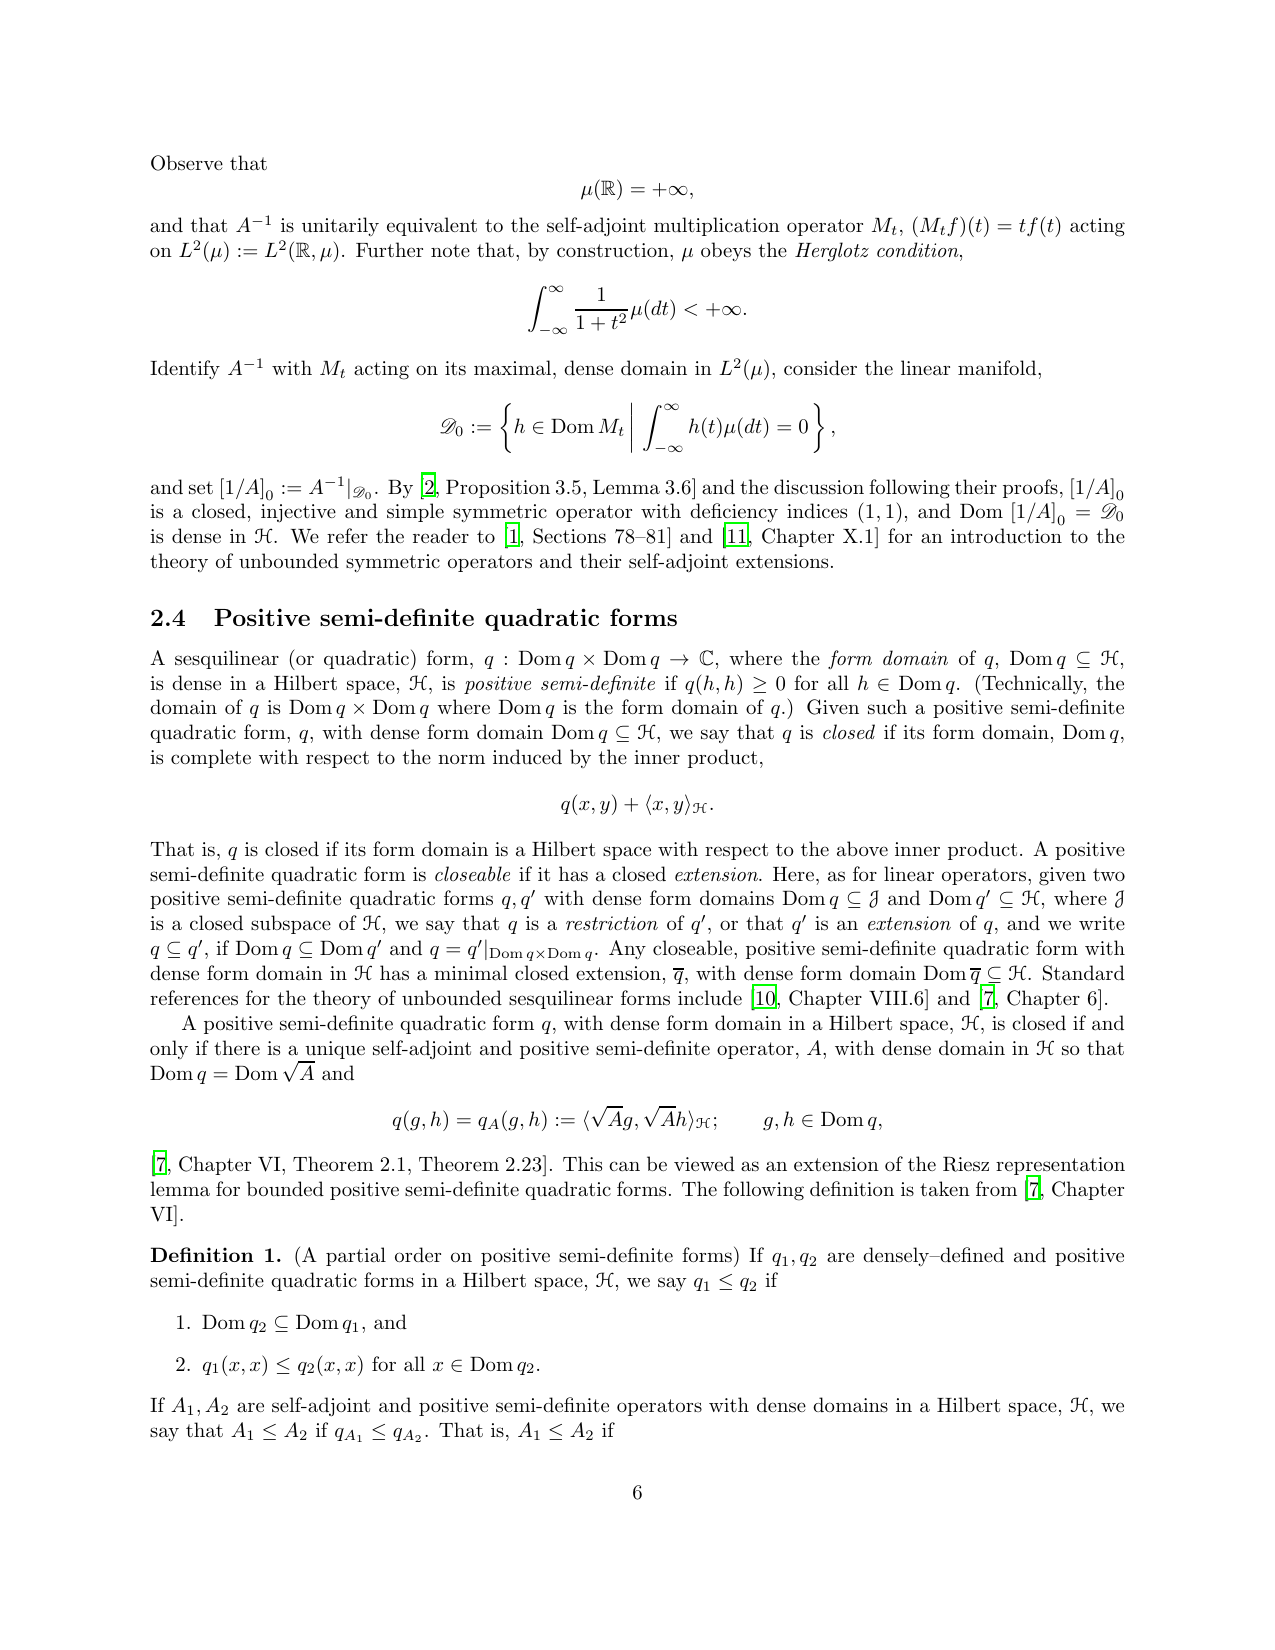
\includegraphics[height=0.78\textheight]{figures/source_construction.png}
\end{center}
\clearpage

\section{A symmetric diagonal model}

Let
\[
 \Hh=\ell^2(\mathbb Z_*),\qquad
 \mathbb Z_*:=\mathbb Z\setminus\{0\},
\]
with canonical basis \((e_k)_{k\in\mathbb Z_*}\), and define
\begin{equation}
 Ae_k=\frac1k e_k.
 \tag{2}
\end{equation}
Then \(A\) is bounded, injective, self-adjoint, and not invertible.  Its
eigenvalues are all simple and tend to zero.  It is multiplicity-free: for
example,
\[
 \xi_k=(1+k^2)^{-1/2}
 \tag{3}
\]
is cyclic.  Indeed, each spectral point \(1/k\) is isolated in
\(\{0\}\cup\{1/j:j\in\mathbb Z_*\}\); a continuous function on this compact
set can select any one coordinate, and polynomial approximation then puts
every \(e_k\) in the cyclic subspace generated by \(\xi\).

For this cyclic vector, the measure used in the paper's construction has
mass
\[
 (1+k^2)|\xi_k|^2=1
\]
at \(k\).  Thus its spectral representation is precisely counting measure
on \(\mathbb Z_*\), and
\begin{equation}
 T=A^{-1}=M_k,\qquad
 \Dom T=\left\{h:\sum_{k\ne0}k^2|h_k|^2<\infty\right\}.
 \tag{4}
\end{equation}
The Herglotz condition holds because
\(\sum_{k\ne0}(1+k^2)^{-1}<\infty\), while the total measure is infinite.
Moreover every \(h\in\Dom T\) is absolutely summable, by Cauchy--Schwarz.
Consequently (1) becomes exactly
\begin{equation}
 \mathcal D_0=\left\{h\in\Dom T:\sum_{k\ne0}h_k=0\right\},
 \qquad T_0=T|_{\mathcal D_0}.
 \tag{5}
\end{equation}
This is not an alternative restriction: it is the restriction specified in
the proof under the cyclic model (3).

\section{The parity splitting}

Let \(R\) be reflection, \((Rh)_k=h_{-k}\), and set
\[
 \Hh_{\rm e}=\ker(R-I),\qquad
 \Hh_{\rm o}=\ker(R+I).
\]
The odd space \(\Hh_{\rm o}\) is infinite-dimensional.  Its elements have
pairwise cancelling coordinates, so
\begin{equation}
 \Dom T\cap\Hh_{\rm o}\subset\mathcal D_0.
 \tag{6}
\end{equation}
In fact the form domain splits as
\begin{equation}
 \mathcal D_0=(\Dom T\cap\Hh_{\rm o})
 \oplus(\mathcal D_0\cap\Hh_{\rm e}).
 \tag{7}
\end{equation}
Multiplication by \(k\) reverses parity, whereas multiplication by \(|k|\)
preserves it.  Hence
\[
 T(\Dom T\cap\Hh_{\rm o})\subset\Hh_{\rm e},
 \qquad
 T(\Dom T\cap\Hh_{\rm e})\subset\Hh_{\rm o}.
\]
It follows that the closed quadratic form
\begin{equation}
 q_0(h,g)=\langle T_0h,T_0g\rangle,
 \qquad h,g\in\mathcal D_0,
 \tag{8}
\end{equation}
is the orthogonal sum of its odd and even restrictions.  On the odd summand,
it is simply
\[
 q_0(h,g)=\langle |T|h,|T|g\rangle.
\]
By uniqueness in the representation theorem for closed positive forms, this
proves the operator identity
\begin{equation}
 |T_0||_{\Hh_{\rm o}}=|T||_{\Hh_{\rm o}},
 \tag{9}
\end{equation}
with equality of the corresponding domains.

\section{A fixed infinite-dimensional subspace of
\texorpdfstring{\(W\)}{W}}

The polar decomposition used by the source is
\[
 T_0=V|T_0|.
\]
The paper proves that \(T_0\) is simple with deficiency indices \((1,1)\),
and its sufficiency argument therefore makes \(V\) a pure isometry of
multiplicity one with \(AV>0\).  We now compute the derived \(W=JV\).

Here
\[
 Je_k=\operatorname{sgn}(k)e_k,
 \qquad |T|e_k=|k|e_k,
 \qquad T=J|T|.
\]
The map \(|T|:\Dom T\cap\Hh_{\rm o}\to\Hh_{\rm o}\) is onto, with bounded
inverse \(|A||_{\Hh_{\rm o}}\).  Given any \(y\in\Hh_{\rm o}\), choose
\(h=|T|^{-1}y\).  Equations (6) and (9), followed by the two polar
decompositions, give
\[
 Vy=V|T_0|h=T_0h=Th=J|T|h=Jy.
\]
Therefore
\begin{equation}
 Wy=JVy=J^2y=y
 \qquad(y\in\Hh_{\rm o}).
 \tag{10}
\end{equation}
Since \(W\) is an isometry, (10) also gives \(W^*y=y\); thus
\(\Hh_{\rm o}\) is a reducing subspace on which \(W\) is the identity.
A pure isometry has \(W^{*n}\to0\) strongly, which is impossible on any
nonzero fixed vector.  Hence \(W\) is not pure.  In fact its identity unitary
part is infinite-dimensional, exactly of the type allowed by Theorem C.

This example uses every defining step of the paper's special construction,
so it answers the stated open problem without weakening ``specific form'' to
an arbitrary pair \((J,V)\).

\begin{thebibliography}{9}
\bibitem{Martin}
R. T. W. Martin,
\emph{On unitary equivalence to a self-adjoint or doubly-positive Hankel
operator}, Concrete Operators \textbf{9} (2022), 114--126,
\href{https://doi.org/10.1515/conop-2022-0132}{doi:10.1515/conop-2022-0132};
arXiv:2205.15925.
\end{thebibliography}

\end{document}
